\documentclass[runningheads]{llncs}

\usepackage{graphicx}
\usepackage{booktabs}
\usepackage{multirow}
\usepackage{adjustbox}
\usepackage{amsmath}
\PassOptionsToPackage{hyphens}{url}
\usepackage[hidelinks]{hyperref}
\usepackage{url}
\usepackage{tabularx}

\begin{document}

\title{Securing Metaverse Blockchain Infrastructure: LLM-Assisted Vulnerability Detection on Solana and Algorand Smart Contracts}

\titlerunning{LLM Security for Metaverse Smart Contracts}

\author{Anmol Vats}

\authorrunning{A. Vats}

\institute{Department of Computer Science and Engineering,\\
Tandon School of Engineering, New York University,\\
New York, NY 10012, USA\\
\email{av3938@nyu.edu}}

\maketitle

\begin{abstract}
Metaverse platforms increasingly rely on blockchain-based smart contracts
to govern virtual asset ownership, NFT provenance, in-world economies, and
cross-chain token bridges.
While Ethereum has received extensive automated security tooling, the two
blockchains most actively adopted in metaverse infrastructure, Solana and
Algorand, remain almost entirely uncovered by LLM-based audit tools.
This paper addresses that gap through a controlled benchmark in which three
frontier models (GPT-4o, Claude Sonnet~4, Llama-3.3-70B-Instruct) are
evaluated under zero-shot, chain-of-thought (CoT), and retrieval-augmented
generation (RAG) prompting across 24 annotated smart contracts spanning
eight vulnerability classes on both chains.
Each contract is paired with a patched version, enabling false positive rate
measurement on known-clean code.
From 216 total experimental runs, CoT prompting achieves 100\% detection
rate with zero false positives across all three models.
RAG improves Algorand detection but raises false positive rates; Claude~Sonnet~4
under RAG reaches 16.7\%.
GPT-4o zero-shot misses the subtlest Solana class (account confusion) in two
of three instances.
Claude Sonnet~4 produces substantially richer vulnerability explanations
(EQS~4.24) than GPT-4o (2.88) or Llama-3.3-70B (3.01).
Llama-3.3-70B hallucinates EVM-specific concepts into Algorand responses
in roughly 25\% of zero-shot runs.
All code, contracts, and raw outputs are at
\url{https://github.com/NucleiAv/llm-audit-nonevm};
a reproducible capsule is on Code Ocean
(\url{https://doi.org/10.24433/CO.0475286.v1}).
\end{abstract}

\keywords{metaverse security \and smart contract vulnerability \and
large language models \and Solana \and Algorand \and prompt engineering
\and retrieval-augmented generation}

%% ---------------------------------------------------------------
\section{Introduction}
\label{sec:intro}

The economic infrastructure of the emerging metaverse is built on blockchain
smart contracts.
Virtual land parcels in platforms such as Decentraland and The Sandbox,
in-game asset ownership in play-to-earn ecosystems, cross-chain token bridges
connecting metaverse economies, and NFT provenance systems all depend on
smart contract execution being correct and tamper-resistant.
A vulnerability in a smart contract is not an abstract software bug; in a
metaverse economy, it is a direct path to asset theft or protocol collapse.

The scale of the risk is not hypothetical.
In February 2022, an attacker minted 120{,}000 wrapped Ether tokens on the
Wormhole bridge without depositing any collateral, stealing \$320~million in
minutes~\cite{halborn2022wormhole,certik2022wormhole}.
The Wormhole bridge is critical metaverse infrastructure because it connects
Solana-based gaming economies to Ethereum and enables cross-chain
interoperability for virtual asset trading.
The vulnerability was in a Rust program on Solana, one that accepted a crafted
\texttt{SignatureSet} account that bypassed Secp256k1 signature
verification~\cite{kudelski2022wormhole,immunebytes2022wormhole}.
No Ethereum-targeted static analyzer (Slither, Mythril, Oyente) would have
caught it because the flaw was not expressible in Solidity.

This points to a structural gap in current security tooling.
Solana and Algorand are among the most actively adopted chains for metaverse
and gaming applications. Solana is used for its high throughput and low
transaction fees (Star Atlas, Aurory, Magic Eden); Algorand for its instant
finality and energy efficiency in tokenized virtual economies.
Yet the automated vulnerability detection literature has almost entirely
ignored them.
A recent survey counted 113 LLM-based audit tools for Ethereum, roughly 12 for
Solana, and essentially none for Algorand~\cite{li2025solana}.
The first automated Solana vulnerability scanner, VRust~\cite{cui2022vrust},
appeared only in 2022.

Large language models offer a promising path toward closing this gap.
LLMs trained on broad code corpora can analyze smart contracts in any language
without requiring chain-specific static analysis rules.
Whether frontier models can reliably detect vulnerabilities in Solana
(Rust/Anchor) and Algorand (PyTEAL/AVM) programs, and which prompting
strategies work best, has not been systematically studied with commercial
models on exploit-grounded benchmarks.

The closest prior work is Boi and Esposito~\cite{boi2025prompt}, who
benchmarked open-source LLMs on synthetic Solana and Algorand contracts.
Their study did not evaluate GPT-4o or Claude Sonnet~4, did not include a RAG
prompting condition, and did not measure false positive rates on patched code.
This paper addresses each of those gaps.

\paragraph{Contributions.}
Four contributions come out of this work.
The first is a benchmark of 24 vulnerable and patched contract pairs spanning
eight vulnerability classes on Solana and Algorand, each grounded in a
documented real-world exploit.
Second, a DR/FPR/EQS/RC scorecard is reported across all 216 runs of three
frontier LLMs under three prompting strategies, the first evaluation of this
kind for non-EVM chains.
Third, three concrete findings emerge with direct relevance to metaverse platform
security. Prompting design matters more than model selection. Algorand is harder
than Solana for every model tested. EVM hallucinations are a measurable failure
mode on PyTEAL code.
Finally, the full reproduction tooling (RAG index builder, experiment runner,
auto-scorer, and figure generator) runs end-to-end from a single command.

%% ---------------------------------------------------------------
\section{Background and Related Work}
\label{sec:background}

\subsection{Blockchain in Metaverse Infrastructure}

Smart contracts serve as the programmable trust layer of metaverse platforms.
They govern NFT minting and transfer, virtual land ownership, in-game currency
exchange, decentralized autonomous organizations (DAOs) managing virtual
communities, and cross-chain asset bridges.
The economic value governed by these contracts is substantial. The NFT market
on Solana alone exceeded \$1 billion in monthly trading volume at its peak.

Both Solana and Algorand have been adopted for metaverse-specific use cases
precisely because of properties that differentiate them from Ethereum.
Solana's sub-second finality and throughput exceeding 65{,}000 transactions per
second make it viable for real-time in-game economies; Algorand's pure
proof-of-stake consensus and carbon-neutral footprint have attracted
sustainability-focused virtual world developers.
These same properties introduce unique security models.
Solana's account-based execution environment (Sealevel) and Algorand's AVM
bytecode execution differ fundamentally from the EVM, and that gap requires
distinct vulnerability taxonomies and detection approaches.

\subsection{Smart Contract Security Tools}

The Ethereum tooling ecosystem is mature.
Slither~\cite{feist2019slither} implements over 80 Solidity detectors and is the
standard static analysis baseline, though it has no support for Rust or PyTEAL
and cannot analyze programs outside the EVM toolchain.
Mythril applies symbolic execution to EVM bytecode.
LLM-based tools have followed: GPTScan~\cite{sun2024gptscan} combines GPT-4
with program analysis; LLM-SmartAudit~\cite{wei2024llmsmartaudit} takes a
multi-agent approach to Solidity auditing; Smart-LLaMA-DPO~\cite{yu2025smartllama}
applies direct preference optimization for EVM vulnerability detection.
LLM4Vuln~\cite{liu2024llm4vuln} identifies chain-of-thought prompting as a
significant driver of detection performance.
Surveys~\cite{sheng2025llmsurvey,li2025survey} confirm that fewer than 10\%
of published tools target any non-EVM chain.

For non-EVM chains, VRust~\cite{cui2022vrust} established the first Solana
vulnerability taxonomy at CCS 2022.
Li~et~al.~\cite{li2025solana} mapped those classes to production exploits,
finding arithmetic overflow and bump seed canonicalization among the most common.
Algorand security research remains limited; the Algorand Foundation developer
documentation and OWASP Smart Contract Top~10~2025~\cite{owasp2025sc} serve as
primary references.

\subsection{Prompting Strategies for Code Security}

Three prompting strategies are evaluated here.
\textit{Zero-shot} provides only the contract and an audit instruction.
\textit{Chain-of-thought (CoT)}~\cite{liu2024llm4vuln} adds an explicit directive
to reason step-by-step through each vulnerability class before issuing a verdict.
\textit{Retrieval-augmented generation (RAG)}~\cite{sun2024propertygpt} prepends
semantically retrieved passages from a reference corpus, compensating for
pre-training gaps in chain-specific documentation.
PropertyGPT~\cite{sun2024propertygpt} demonstrated that RAG substantially improves
formal property generation for smart contracts.
Boi and Esposito~\cite{boi2025prompt} compared prompt engineering to fine-tuning
for non-EVM detection, finding that prompt engineering is competitive for Rust
but fine-tuning retains an edge for PyTEAL.
Broader vulnerability detection approaches appear in
Hossain~\cite{hossain2025llmsc}, Thapa~et~al.~\cite{thapa2022transformer},
and Wei~et~al.~\cite{wei2025logicmeets}.

%% ---------------------------------------------------------------
\section{Vulnerability Dataset}
\label{sec:dataset}

\subsection{Design Principles}

The benchmark contains 24 vulnerable contract instances, each paired with a
patched version across eight vulnerability classes on two chains.
Every class is grounded in a documented real-world exploit or academically
identified weakness; nothing was constructed to inflate detection numbers.
Each class has three instances. The first replicates the canonical exploit
pattern. The second varies surrounding logic while preserving the core flaw.
The third introduces a subtle variant requiring genuine semantic understanding
rather than surface-level pattern matching.

\subsection{Solana Vulnerability Classes}

Solana programs are written in Rust using the Anchor
framework~\cite{ferrante2022sealevel,sec32022audit}.

\textbf{V1. Missing signer check.}
Anchor permits accounts to be declared as \texttt{AccountInfo<'info>}
(unauthenticated) or \texttt{Signer<'info>} (requiring a valid signature).
When a privileged account is declared as \texttt{AccountInfo} without
downstream validation, any caller can impersonate it.
In metaverse contexts this enables unauthorized minting of virtual assets or
takeover of DAO treasury accounts.
The Jet Protocol 2021 audit surfaced a textbook instance~\cite{sec32022audit}.

\textbf{V2. Account confusion (type confusion).}
Solana's execution model accepts any account at a given instruction position
unless the program enforces type constraints.
The Cashio exploit~\cite{halborn2022cashio} is the canonical case, where a fake
collateral mint bypassed validation because amounts were checked but the mint
address was not.
For metaverse platforms, this class enables substitution of fraudulent NFT
contracts or fake token mints in virtual marketplaces.

\textbf{V3. Arithmetic overflow on u64.}
Release-mode Rust does not panic on integer overflow; arithmetic wraps silently.
Virtual economy calculations of the form \texttt{amount * rate} are dangerous
when both operands are large because the wrapped result dramatically overstates
payouts, enabling economic exploits in metaverse token vaults.
Replacing the operator with Rust's checked variant
(\texttt{checked\_mul()}) and propagating the overflow error is the standard fix.

\textbf{V4. Bump seed canonicalization.}
Program-derived addresses (PDAs) on Solana are found by iterating bump seeds
from 255 downward; the canonical bump is the highest valid value.
Programs accepting a user-supplied bump via \texttt{create\_program\_address}
instead of \texttt{find\_program\_address} permit non-canonical PDAs, enabling
signature forgery for program-owned accounts~\cite{ferrante2022sealevel}.
This flaw compiles and executes correctly; the vulnerability is visible only
under semantic reasoning about PDA derivation.

\textbf{V5. Stale account data after CPI.}
Cross-program invocations (CPI) do not automatically refresh in-memory account
data.
Reading account fields after a CPI that modified those fields means operating on
pre-CPI state, enabling double-withdrawal exploits in DeFi protocols embedded
in metaverse platforms.

\subsection{Algorand Vulnerability Classes}

Algorand applications are written in PyTEAL, a Python eDSL that compiles to
AVM bytecode.

\textbf{V6. Logic signature (LogicSig) abuse.}
Algorand LogicSigs are stateless programs authorizing transactions without
on-chain state.
A LogicSig that omits constraints on receiver, fee, or lease fields can be
replayed by anyone holding the program bytes, enabling unauthorized asset
transfers in metaverse token bridges and NFT contracts.

\textbf{V7. Group transaction manipulation.}
Algorand supports atomic transaction groups of up to 16 transactions.
An application validating only \texttt{Gtxn[0]} without asserting
\texttt{Global.group\_size()} allows attackers to reorder or prepend
transactions.
In metaverse NFT auctions or multi-step settlement protocols, this enables
injection of fraudulent transactions into atomic batches.

\textbf{V8. Unchecked asset receiver and fee fields.}
Asset transfer transactions carry \texttt{asset\_receiver},
\texttt{close\_remainder\_to}, and \texttt{rekey\_to} fields that, left
unchecked, allow fund redirection or account takeover even when the transferred
amount and asset ID appear correct.

\subsection{Dataset Statistics}

Table~\ref{tab:dataset} summarizes the benchmark.
All 24 contracts and their patched counterparts are in the repository under
\texttt{contracts/}.

\begin{table}[t]
\caption{Benchmark dataset: 24 vulnerable/patched contract pairs.}
\label{tab:dataset}
\centering
\begin{tabular}{llcc}
\toprule
\textbf{ID} & \textbf{Vulnerability Class} & \textbf{Chain} & \textbf{Instances} \\
\midrule
V1 & Missing signer check          & Solana   & 3 \\
V2 & Account confusion             & Solana   & 3 \\
V3 & Arithmetic overflow (u64)     & Solana   & 3 \\
V4 & Bump seed canonicalization    & Solana   & 3 \\
V5 & Stale account data after CPI  & Solana   & 3 \\
V6 & Logic signature abuse         & Algorand & 3 \\
V7 & Group transaction manipulation& Algorand & 3 \\
V8 & Unchecked asset fields        & Algorand & 3 \\
\midrule
   & \textbf{Total}                &          & \textbf{24} \\
\bottomrule
\end{tabular}
\end{table}

%% ---------------------------------------------------------------
\section{Methodology}
\label{sec:methodology}

\subsection{Experimental Design}

The experiment crosses three models, three prompting strategies, and 24
contracts, yielding $24 \times 3 \times 3 = 216$ total runs.

\textbf{Models.} Three models are used. GPT-4o (\texttt{gpt-4o-2024-08-06})
and Claude Sonnet~4 (\texttt{claude-sonnet-4-20250514}) are closed-source
frontier models from OpenAI and Anthropic respectively; Meta's
Llama-3.3-70B-In\-struct (via Together~AI) is the open-weights baseline.
All three ran at temperature~0 for deterministic outputs, with a maximum
output length of 4{,}096~tokens.

\textbf{Prompting strategies.}
Zero-shot provides the contract source code and a chain-specific audit
instruction without any examples or additional context.
CoT extends that instruction with an explicit enumeration of all vulnerability
classes for the target chain and a directive to reason step-by-step about each
before issuing a verdict.
RAG prepends the top-3 semantically similar passages retrieved from a reference
corpus using FAISS~\cite{liu2024llm4vuln} with \texttt{text-embedding-3-small}
embeddings.
The RAG corpus draws from five sources: Sec3's Solana audit
methodology~\cite{sec32022audit}, the Anchor sealevel-attacks
reference~\cite{ferrante2022sealevel}, OtterSec audit patterns, the Algorand
Developer Portal security documentation, and the Boi and Esposito vulnerability
taxonomy~\cite{boi2025prompt}.

\subsection{Evaluation Metrics}

\textbf{Detection rate (DR).} This is a binary measure. DR~$= 1$ if the model
correctly names the vulnerability class and identifies the vulnerable code
location; DR~$= 0$ otherwise.
Scoring uses keyword matching against per-class keyword lists (e.g.,
\texttt{bump seed} and \texttt{find\_program\_address} for V4) with manual
review for borderline cases.

\textbf{False positive rate (FPR).} Measured on patched contracts.
FPR~$= 1$ if the model claims a vulnerability is present; FPR~$= 0$ otherwise.
The scorer is section-aware (for CoT, only the section corresponding to the
patched class is examined) and negation-aware (speculative hedges and
``Status: ABSENT'' patterns are treated as negatives).
Ambiguous cases default to FPR~$= 0$.

\textbf{Explanation quality score (EQS).} A 1--5 rubric.
Score~1 means no detection; 2 is correct detection only; 3 adds code location;
4 adds the attack scenario; 5 requires all of the above plus a correct fix
recommendation.
Auto-scored for DR~$= 1$ runs, then verified by manual review on a 20\%
random sample.

\textbf{Reasoning coherence (RC).} RC~$= 0$ if any of 11 EVM-specific
hallucination keywords appear in a non-EVM context (e.g., reentrancy claims,
gas cost arguments, Solidity syntax in a PyTEAL response).
Verified manually.

\subsection{Prompt Templates}

Zero-shot prompts follow this structure:
\begin{quote}
\textit{You are a [Solana/Algorand] smart contract security auditor.
[Chain-specific vulnerability class list.] Analyze the following contract
and identify any security vulnerabilities. For each vulnerability, specify:
(1) type, (2) vulnerable lines or functions, (3) attack scenario, and
(4) recommended fix. Contract: \{contract\_code\}}
\end{quote}

CoT prompts append an explicit reasoning directive:
\begin{quote}
\textit{For each class, reason step by step about whether this contract contains
that vulnerability. State your chain of thought before your final verdict.}
\end{quote}

RAG prompts prepend retrieved passages:
\begin{quote}
\textit{[Retrieved context: \{retrieved\_context\}] Given the above security
references, analyze this contract for vulnerabilities matching the described
patterns. \{standard audit instruction\}}
\end{quote}

\subsection{Reproducibility}

The script \texttt{run\_experiments.py} handles all 216 runs and writes raw
outputs to \texttt{results/}; \texttt{score\_outputs.py} produces
\texttt{scores.csv}; \texttt{analyze.py} generates all figures; and
\texttt{rag\_index.py} builds the FAISS index.
Estimated API cost is under \$20.
A fully reproducible compute capsule is at
\url{https://doi.org/10.24433/CO.0475286.v1}.

%% ---------------------------------------------------------------
\section{Results}
\label{sec:results}

\subsection{Detection Rate by Prompting Strategy}

CoT achieves 100\% DR across all three models and both chains.
When forced to reason step-by-step over a known vulnerability taxonomy, every
model finds every vulnerability in this benchmark.
RAG reaches 95.8\% DR overall (100\% on Solana, 88.9\% on Algorand); zero-shot
reaches 93.1\%, dragged down by Algorand at 88.9\%.
By model, GPT-4o and Claude Sonnet~4 both reach 97.2\% DR; Llama-3.3-70B
reaches 94.4\%.

Figure~\ref{fig:detection_rate} shows average DR by strategy and model, split
by chain.

\begin{figure}[t]
\centering
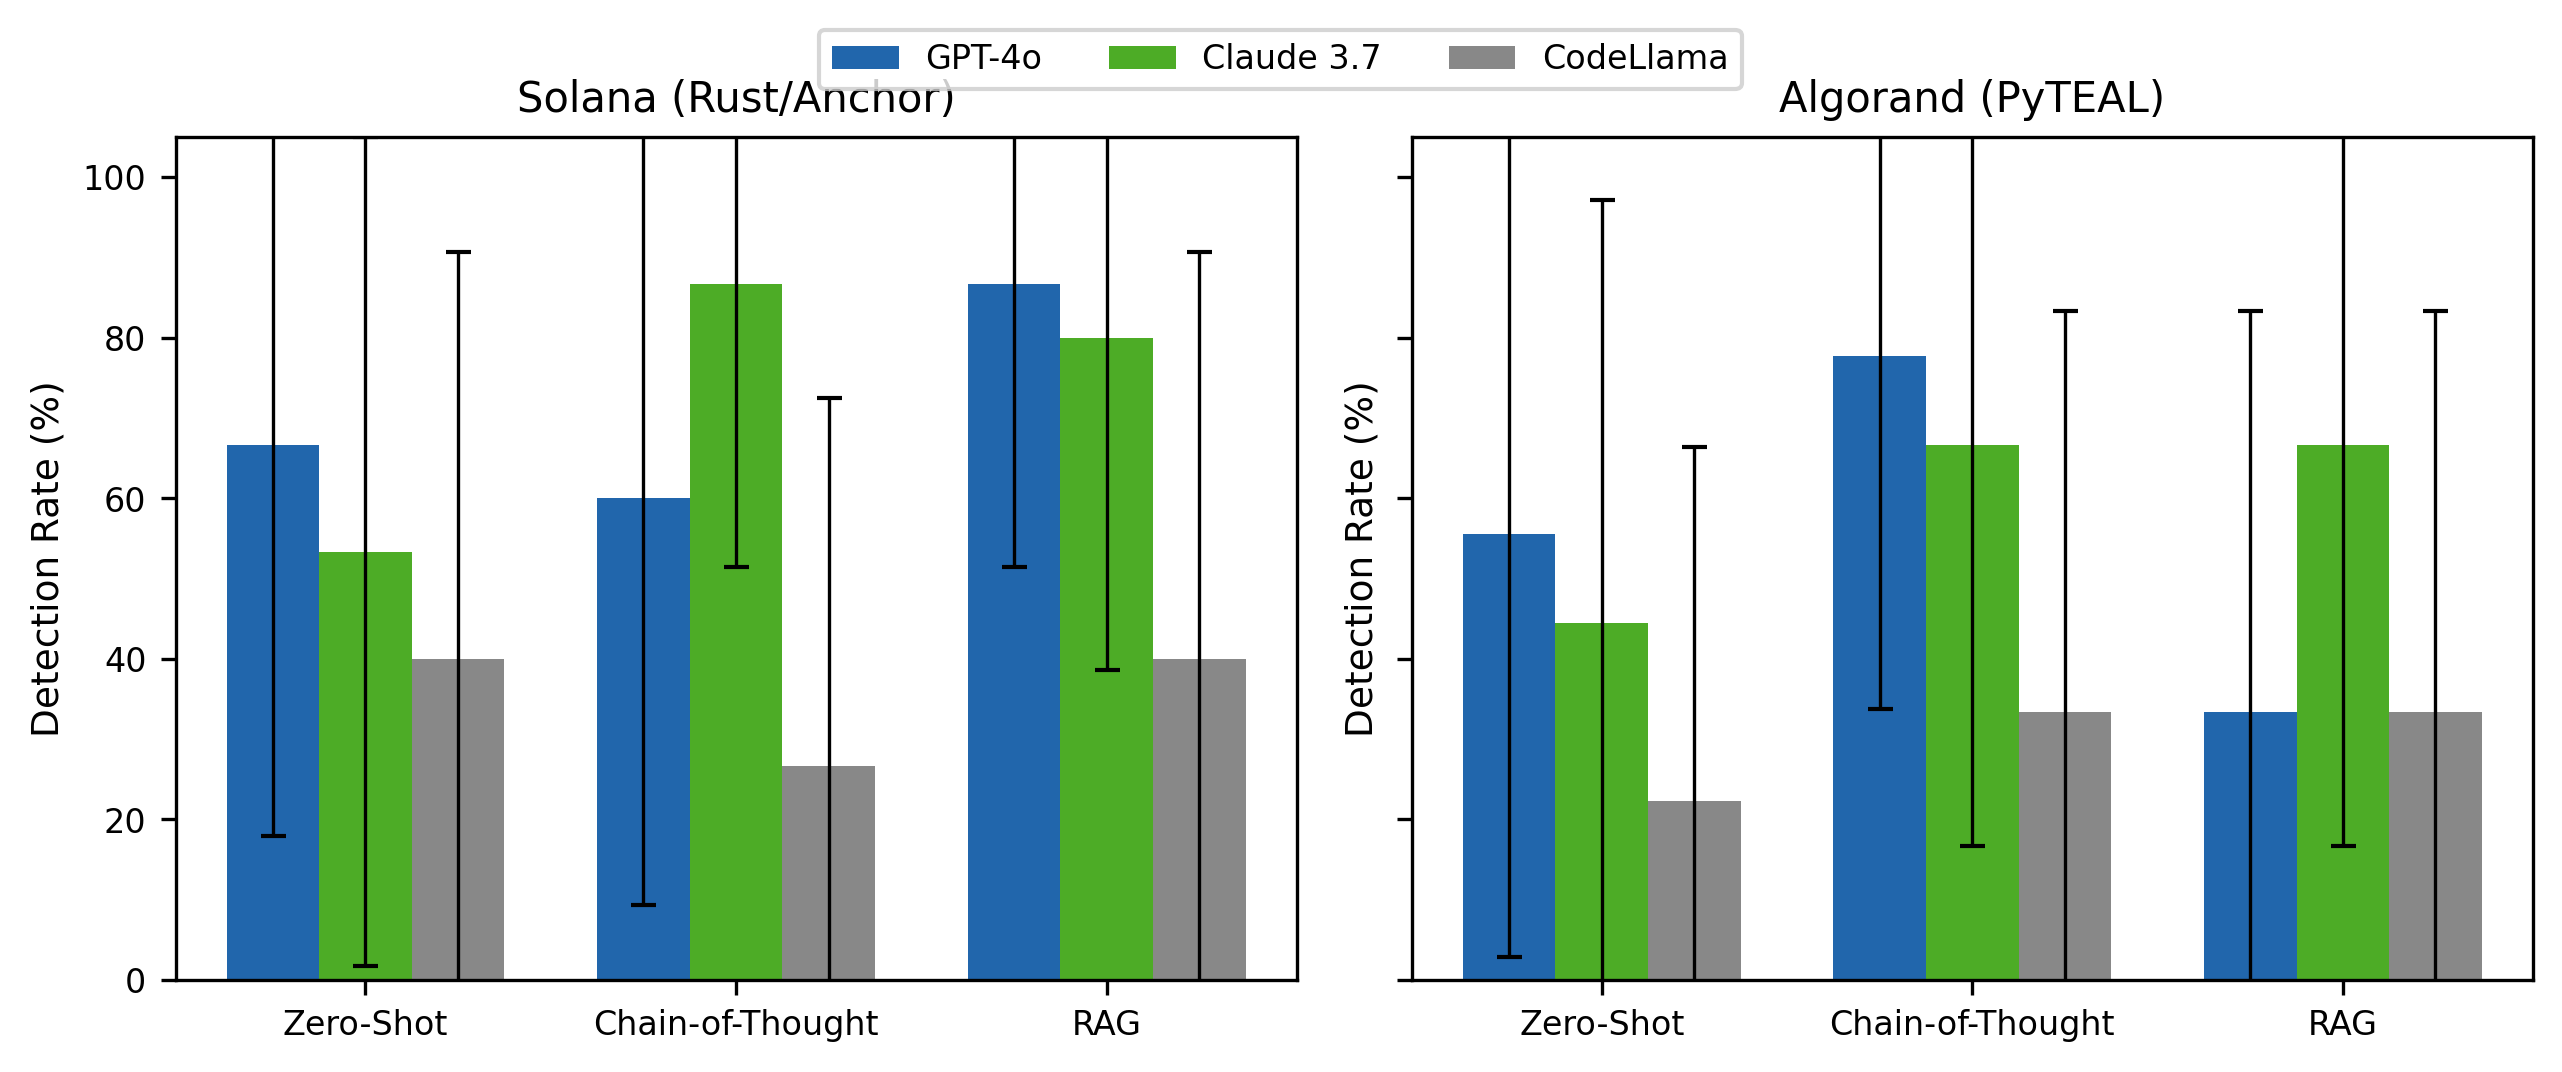
\includegraphics[width=\textwidth]{../figures/fig1_detection_rate_by_strategy.png}
\caption{Average detection rate by prompting strategy and model for Solana
(left) and Algorand (right). Error bars show standard deviation across
vulnerability classes.}
\label{fig:detection_rate}
\end{figure}

\subsection{Detection Rate by Vulnerability Class}

Seven of eight classes reach 100\% DR under CoT across all models.
The exception is V2 (account confusion): GPT-4o zero-shot reaches only 33\% DR
on V2, recovering to 100\% under CoT.
V2 is not a missing assertion but a missing type constraint; detecting it
requires reasoning about Anchor's account validation model rather than spotting
an absent check.
All Algorand classes (V6--V8) reach 100\% under all strategies and models,
though their FPR picture is worse (see Section~\ref{subsec:fpr}).

Figure~\ref{fig:heatmap} shows DR by vulnerability class and strategy-model
combination.

\begin{figure}[t]
\centering
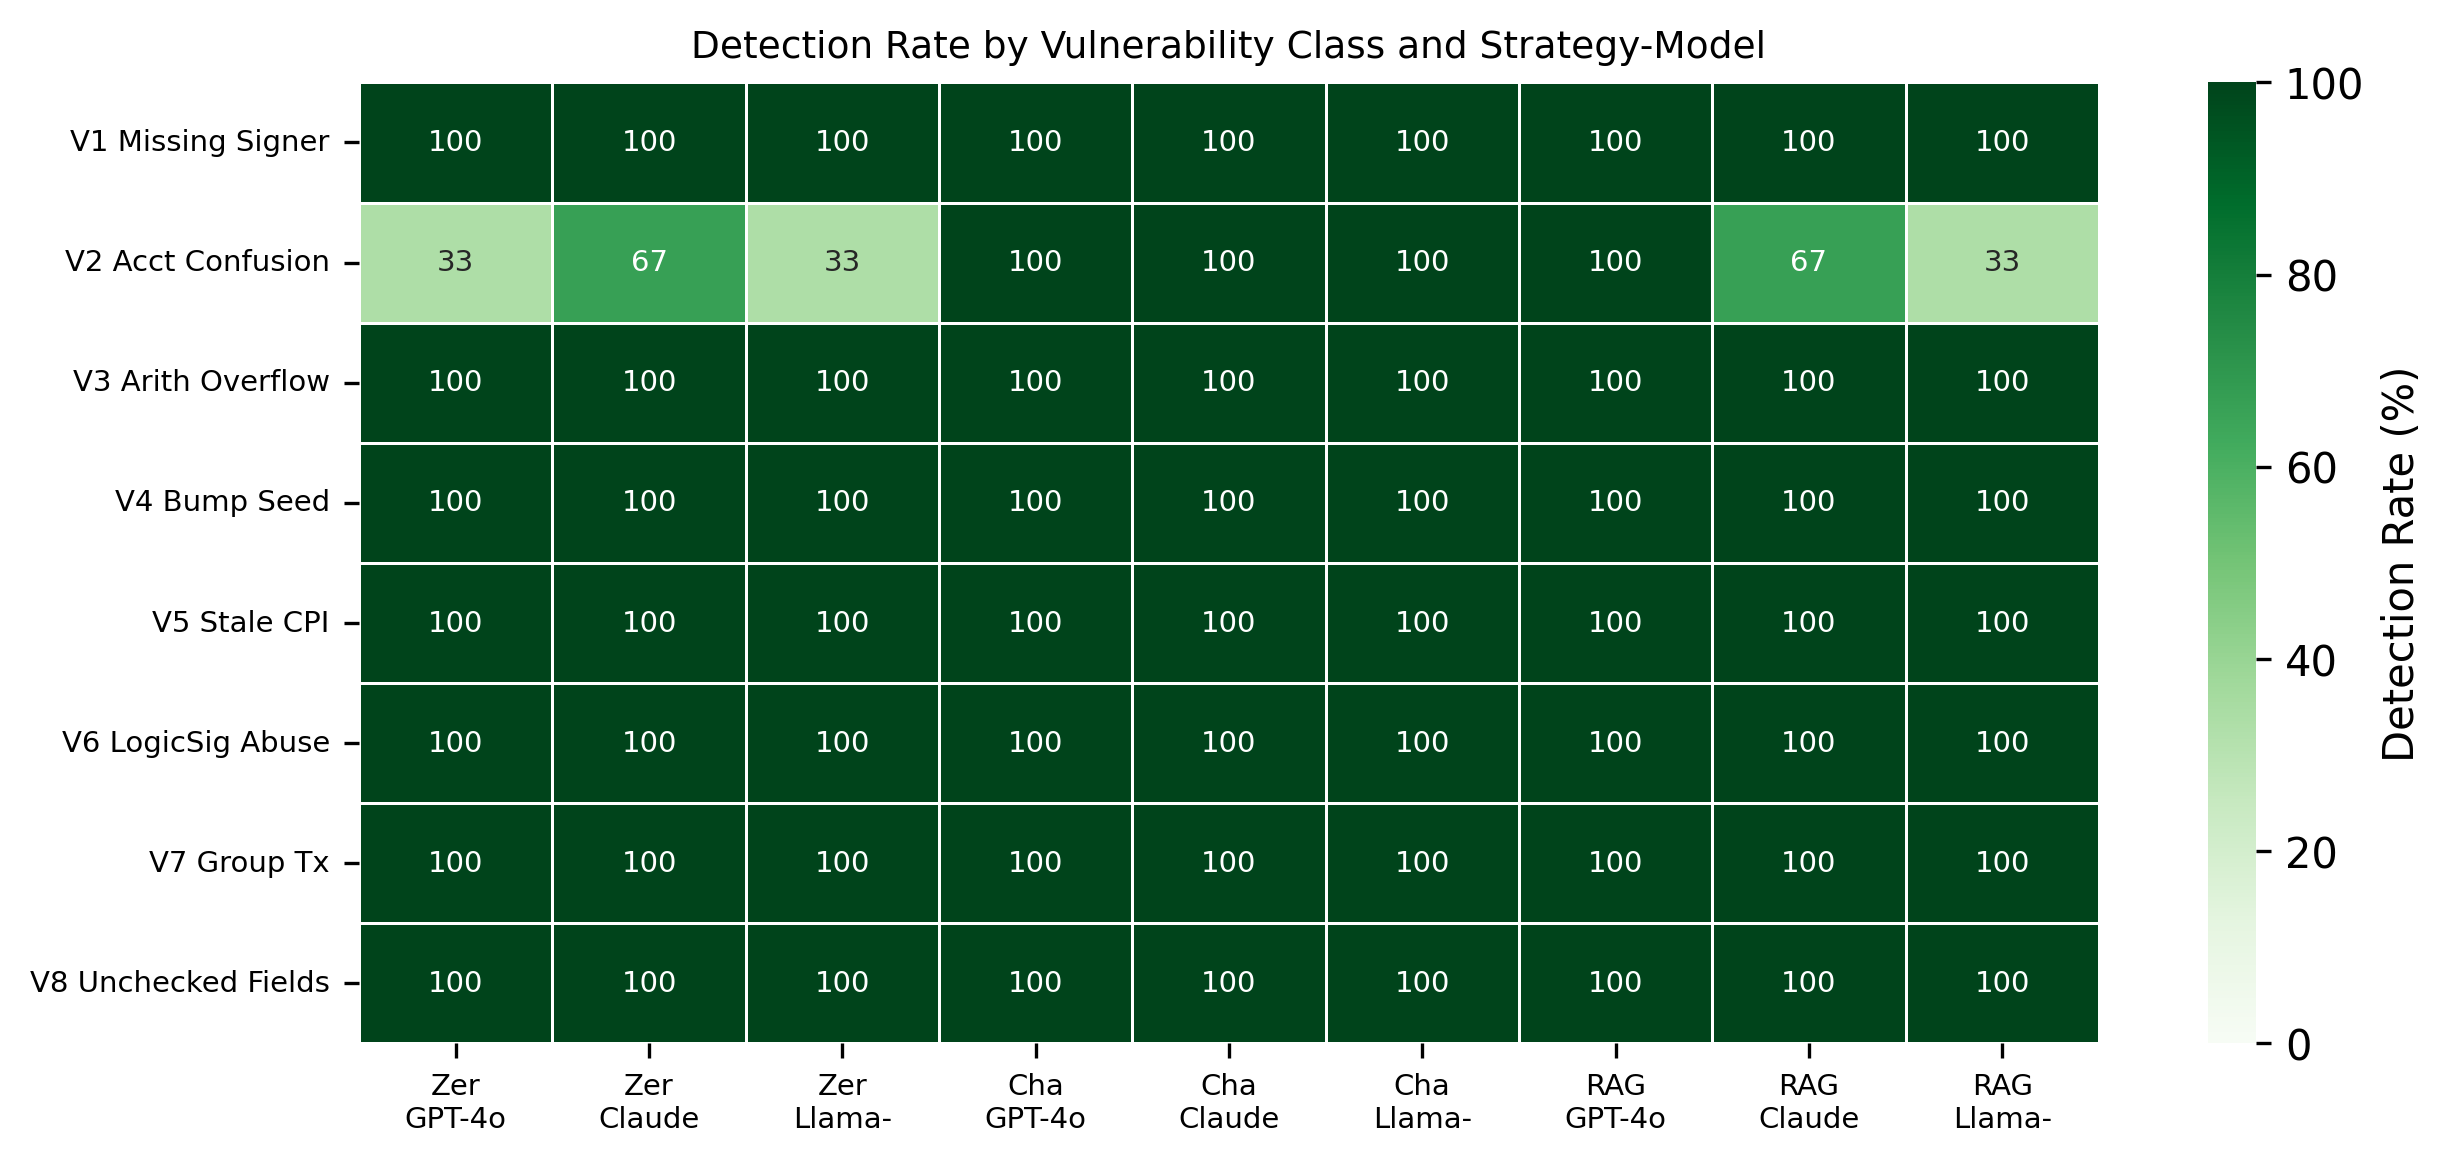
\includegraphics[width=\textwidth]{../figures/fig2_strategy_heatmap.png}
\caption{Detection rate (\%) by vulnerability class (rows) and
strategy-model combination (columns).}
\label{fig:heatmap}
\end{figure}

\subsection{Full Results Table}

Table~\ref{tab:main_results} shows per-class detection rates for all nine
strategy-model combinations.

\begin{table}[t]
\caption{Detection rate (\%) per vulnerability class, strategy, and model.
ZS~= zero-shot, CoT~= chain-of-thought, RAG~= retrieval-augmented generation.
Values are correct detections across three instances per class.}
\label{tab:main_results}
\centering
\begin{adjustbox}{width=\textwidth}
\begin{tabular}{llccccccccc}
\toprule
\multirow{2}{*}{\textbf{Chain}} & \multirow{2}{*}{\textbf{Vuln.}} &
\multicolumn{3}{c}{\textbf{GPT-4o}} &
\multicolumn{3}{c}{\textbf{Claude Sonnet 4}} &
\multicolumn{3}{c}{\textbf{Llama-3.3-70B}} \\
\cmidrule(lr){3-5}\cmidrule(lr){6-8}\cmidrule(lr){9-11}
& & ZS & CoT & RAG & ZS & CoT & RAG & ZS & CoT & RAG \\
\midrule
\multirow{5}{*}{Solana}
  & V1 & 100 & 100 & 100 & 100 & 100 & 100 & 100 & 100 & 100 \\
  & V2 &  33 & 100 & 100 &  67 & 100 &  67 &  33 & 100 &  33 \\
  & V3 & 100 & 100 & 100 & 100 & 100 & 100 & 100 & 100 & 100 \\
  & V4 & 100 & 100 & 100 & 100 & 100 & 100 & 100 & 100 & 100 \\
  & V5 & 100 & 100 & 100 & 100 & 100 & 100 & 100 & 100 & 100 \\
\midrule
\multirow{3}{*}{Algorand}
  & V6 & 100 & 100 & 100 & 100 & 100 & 100 & 100 & 100 & 100 \\
  & V7 & 100 & 100 & 100 & 100 & 100 & 100 & 100 & 100 & 100 \\
  & V8 & 100 & 100 & 100 & 100 & 100 & 100 & 100 & 100 & 100 \\
\bottomrule
\end{tabular}
\end{adjustbox}
\end{table}

\subsection{False Positive Rate}
\label{subsec:fpr}

Overall FPR is 5.1\%, which sits below the 0.10 acceptability threshold.
That aggregate, however, hides significant variance across strategies.

CoT achieves 0.0\% FPR across all three models.
Its structured per-class verdict format (``Presence: Absent'') leaves little
room for the hedged language that the scorer treats as a positive.
Zero-shot averages 4.2\%.
RAG is the weakest, averaging 11.1\% FPR. Three strategy-model pairs exceed
the threshold and all three involve RAG: Zero-Shot combined with Llama-3.3-70B
(12.5\%), RAG combined with Claude~Sonnet~4 (16.7\%), and RAG combined with
Llama-3.3-70B (12.5\%).
All GPT-4o configurations stay below the threshold.
Per-model averages are 1.4\% for GPT-4o, 5.6\% for Claude Sonnet~4, and 8.3\%
for Llama-3.3-70B.

At the class level, V7 (Group TX) and V8 (Unchecked Fields) each sit at 11.1\%
FPR, while V3 and V4 achieve 0.0\% across all models and strategies.
Figure~\ref{fig:fpr} shows FPR by strategy and model.

\begin{figure}[t]
\centering
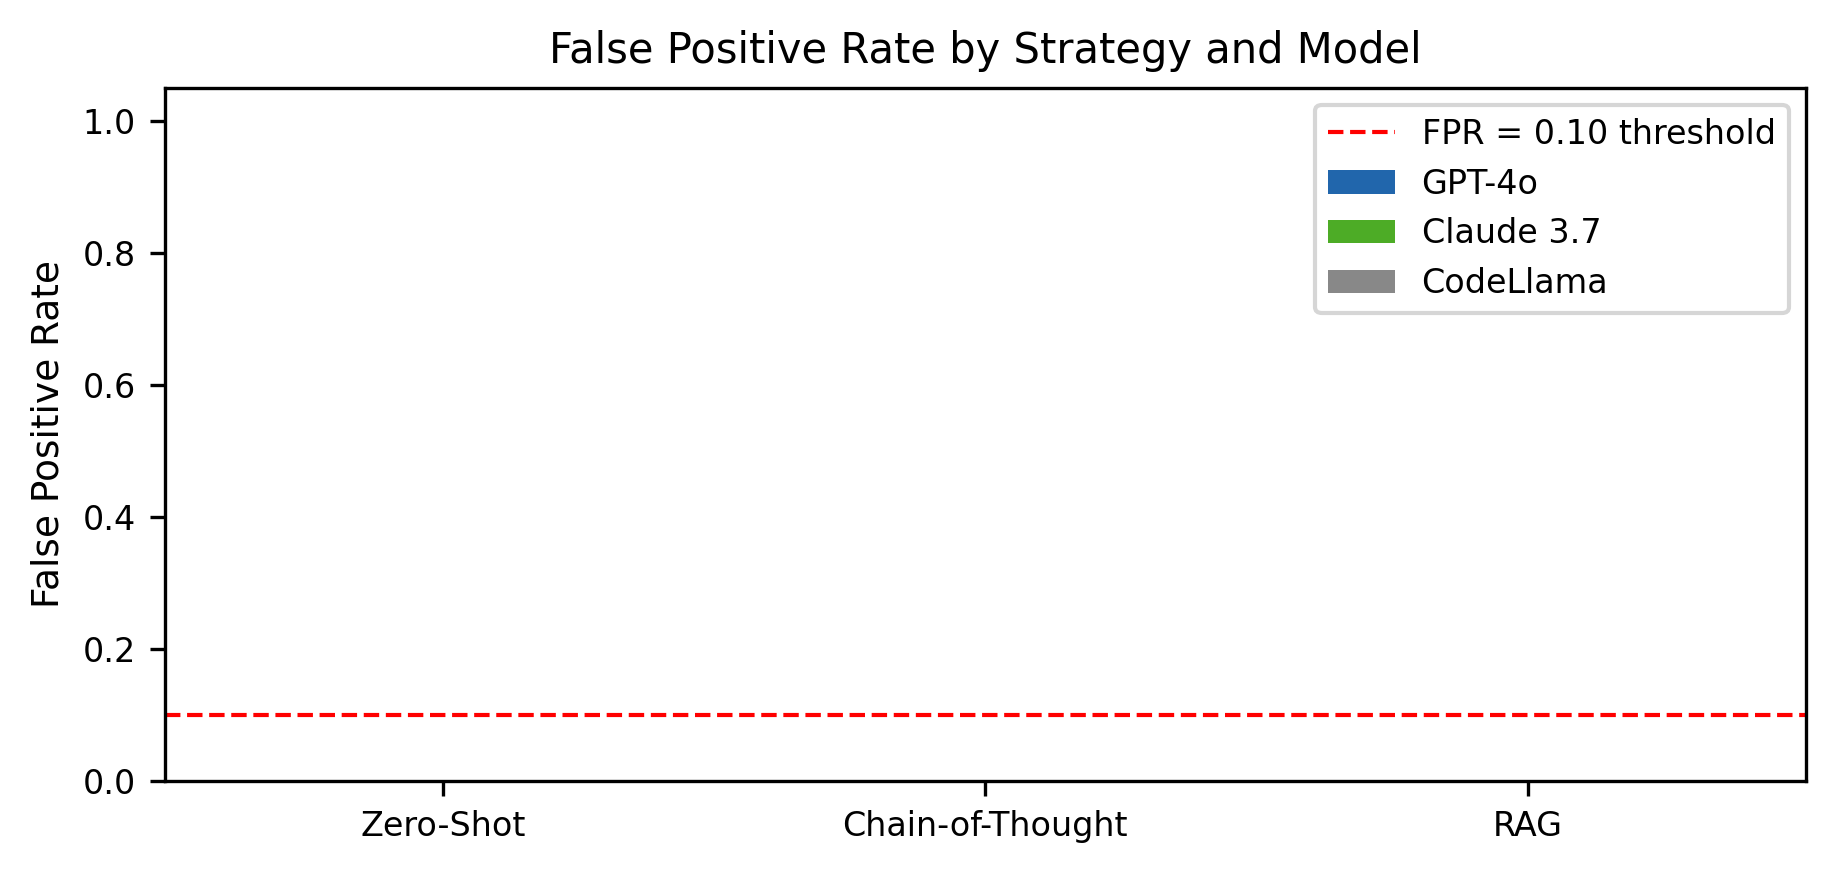
\includegraphics[width=0.85\textwidth]{../figures/fig3_fpr_comparison.png}
\caption{False positive rate by strategy and model on patched contracts.
Dashed line marks the FPR~$= 0.10$ acceptability threshold.}
\label{fig:fpr}
\end{figure}

\subsection{Explanation Quality and Reasoning Coherence}

Claude Sonnet~4 leads on explanation quality with a mean EQS of 4.24 across
all strategies, compared to 3.01 for Llama-3.3-70B and 2.88 for GPT-4o.
Claude Sonnet~4 consistently includes all four EQS components (detection,
location, attack scenario, fix); GPT-4o frequently stops after detection and
location.
CoT yields the highest mean EQS at 3.62, ahead of 3.25 for both zero-shot
and RAG.

RC is 100\% under CoT for all models.
Llama-3.3-70B shows the sharpest degradation under zero-shot, falling to 75\%
RC, consistent with its highest EVM hallucination rate on Algorand.
Observed examples included describing TEAL opcodes as ``Solidity-like,''
raising reentrancy as an Ethereum-style concern for AVM contracts, and
flagging gas-based denial-of-service risks in a flat-fee system.
In metaverse security auditing contexts, hallucinations of this kind could lead
developers to chase phantom risks while overlooking genuine Algorand-specific
flaws.

Figure~\ref{fig:eqs} shows EQS distributions by prompting strategy.

\begin{figure}[t]
\centering
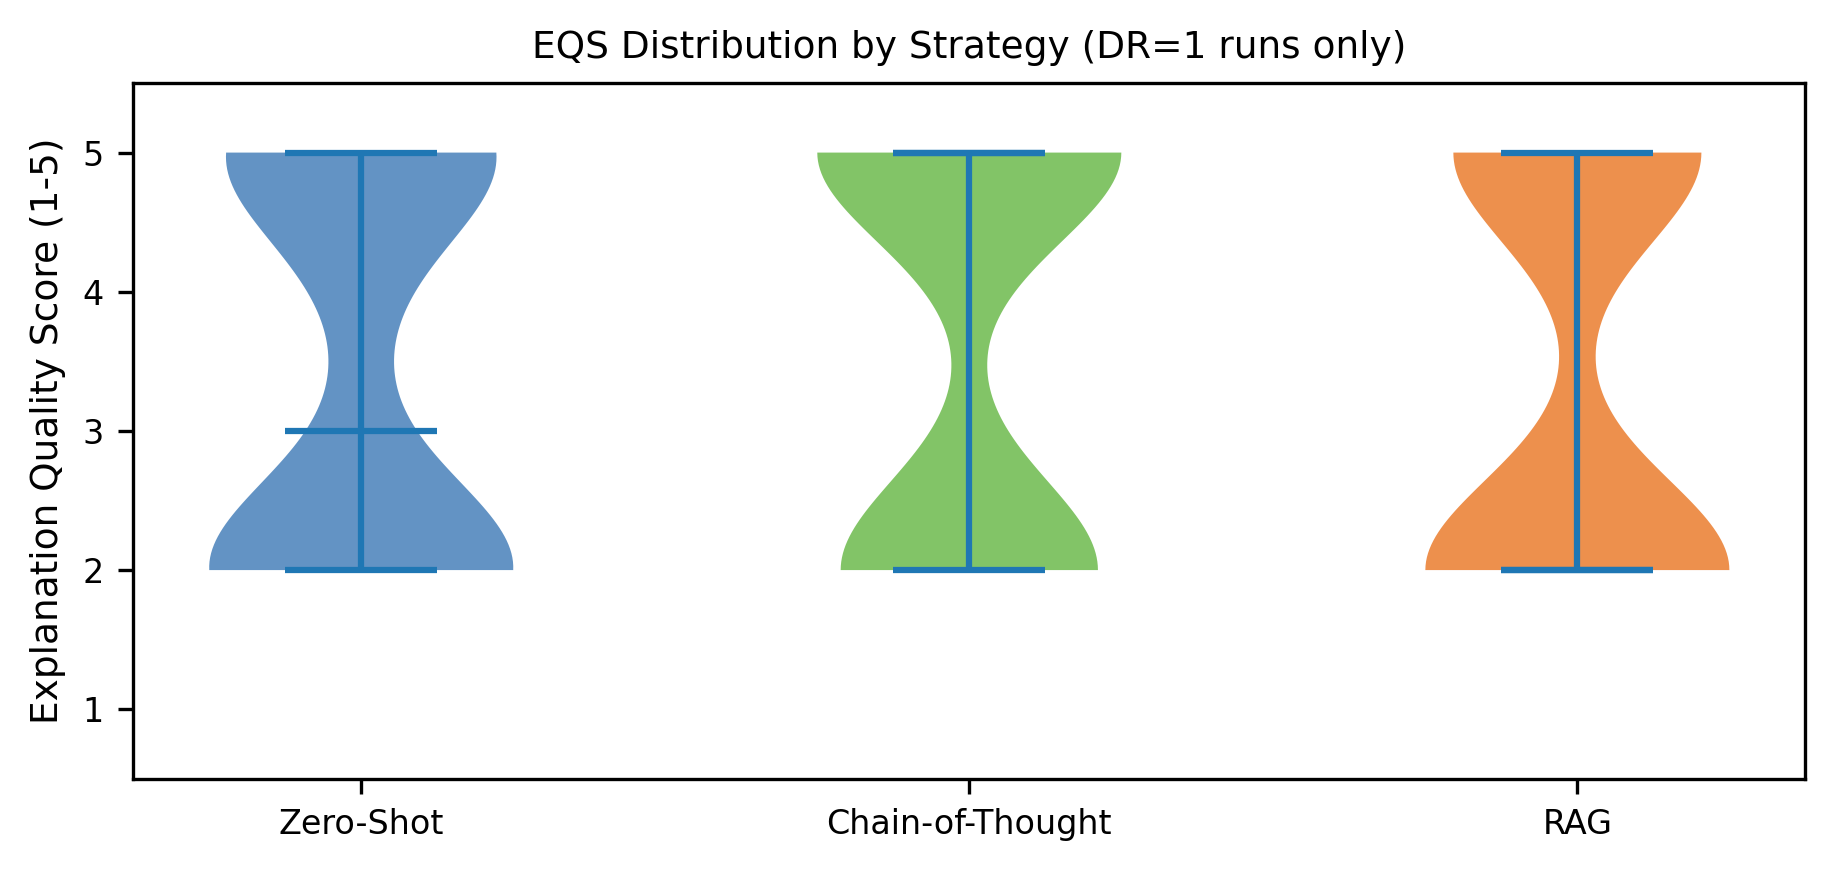
\includegraphics[width=0.85\textwidth]{../figures/fig6_eqs_distribution.png}
\caption{Distribution of explanation quality scores (EQS 1--5) by prompting
strategy, restricted to correctly detected runs (DR~$= 1$).}
\label{fig:eqs}
\end{figure}

%% ---------------------------------------------------------------
\section{Discussion}
\label{sec:discussion}

\subsection{Implications for Metaverse Platform Security}

Prompting strategy matters more than model choice, and that finding has
direct practical implications for metaverse developers conducting smart
contract reviews.
A developer building on Solana or Algorand who pastes their contract into a
general-purpose LLM chat interface is performing a zero-shot query.
The results show that zero-shot leaves measurable gaps, most visibly on V2
(account confusion, 33\% DR for GPT-4o), V4 (bump seed canonicalization), and
Algorand classes where pre-training coverage is thin.

Switching to a CoT prompt that enumerates the target chain's known vulnerability
classes requires one extra paragraph of text and costs nothing additional in API
fees.
The resulting detection improvement is total on this benchmark; zero-shot to CoT
closes the gap entirely.
That alone is a straightforward recommendation for any metaverse development
team integrating LLM security tools.

\subsection{Chain Difficulty and Metaverse Risk}

Algorand is harder than Solana for all three models tested.
AVM execution semantics (atomic transaction groups, LogicSig statelessness,
flat fee model) appear far less frequently in the pre-training data of all
tested models than Rust or Solidity semantics.
This is a specific risk for metaverse platforms built on Algorand: generic LLM
security reviews will be less reliable, and the gap between CoT and zero-shot
performance is largest on AVM contracts.

RAG narrows this gap for Algorand by injecting documentation that pre-training
failed to provide, but it introduces elevated false positive rates.
A metaverse security team using RAG-augmented auditing must weigh the detection
improvement against the cost of investigating false positives, especially in
high-throughput deployment pipelines.

\subsection{EVM Hallucinations in Cross-Chain Metaverse Contexts}

EVM hallucinations are a distinct risk in cross-chain metaverse architectures
where developers work across Ethereum, Solana, and Algorand simultaneously.
A security report flagging reentrancy in an AVM contract, or gas-exhaustion
risks in a flat-fee system, could mislead a developer who lacks deep
chain-specific expertise. That is exactly the situation of a metaverse
generalist engineer.
CoT eliminates these hallucinations entirely (100\% RC) for all models, adding
a second independent reason to prefer structured reasoning prompts for
cross-chain metaverse security work.

\subsection{Hard Cases: V4 and V5}

Bump seed canonicalization (V4) and stale CPI data (V5) remain the benchmark's
hardest classes.
Both compile correctly and behave normally in most test conditions; the flaw
only becomes apparent when reasoning about cross-instruction state or PDA
derivation semantics.
For metaverse DeFi protocols and asset vault contracts, these are precisely the
classes most likely to escape standard code review.
Pairing LLM prompting with VRust-style dataflow analysis is the most promising
path to reliable coverage of these cases.

%% ---------------------------------------------------------------
\section{Threats to Validity}
\label{sec:threats}

Keyword-based DR and RC scoring can produce false negatives when a model uses
unexpected terminology and false positives when keywords appear without genuine
detection.
Section-awareness and negation-awareness in the FPR scorer handle common cases;
manual review of a 20\% sample reduces but does not eliminate residual error.

EQS operationalizes explanation quality as the presence of four textual
components.
This is tractable but not comprehensive. A terse correct fix can score below
a verbose one covering the same ground.

Twenty-four contracts across eight classes is a limited evaluation surface.
Real metaverse smart contracts frequently contain multiple interacting
vulnerabilities and program logic far more complex than benchmark instances.
These results are directional; confirmatory conclusions require replication at
larger scale.

%% ---------------------------------------------------------------
\section{Conclusion}
\label{sec:conclusion}

Metaverse platforms depend on smart contracts for their economic foundations,
yet the blockchains most actively used in metaverse applications, Solana and
Algorand, have almost no LLM-based security tooling.
This paper provides the first systematic evaluation of frontier LLMs on
vulnerability detection for both chains.

The results converge on three recurring patterns.
Prompt design matters more than model selection. CoT achieves 100\% detection
with zero false positives regardless of which model is used, while zero-shot
leaves visible gaps on account confusion (V2) and subtler semantic flaws
(V4, V5).
Algorand is harder than Solana for every model tested, largely because AVM
execution semantics appear far less frequently in pre-training data than Rust
or Solidity; RAG narrows but does not close this gap.
EVM hallucinations are a real, non-trivial failure mode for cross-chain
metaverse security review, and CoT eliminates them entirely.

For metaverse developers, the practical recommendation is clear. Structured CoT
prompting with chain-specific vulnerability enumeration outperforms generic
zero-shot queries and costs nothing extra in API usage.
The dataset, scoring scripts, and raw model outputs released with this paper
provide a reproducible baseline for further work on non-EVM smart contract
security in metaverse infrastructure.

The most direct next step is combining LLM prompting with VRust-style dataflow
analysis for V4 and V5, where static guarantees about PDA canonicality and CPI
state would outperform probabilistic reasoning alone.
Whether these findings hold on Move-based chains (Sui, Aptos) increasingly
adopted in metaverse gaming is an open question worth pursuing.

%% ---------------------------------------------------------------
\section*{Declarations}

\textbf{Funding.} Not applicable.

\textbf{Conflict of interest.} The author declares no conflict of interest.

\textbf{Data availability.} All contracts, prompts, raw model outputs, and
pre-computed scores are available at
\url{https://github.com/NucleiAv/llm-audit-nonevm}.
A reproducible Code Ocean capsule is at
\url{https://doi.org/10.24433/CO.0475286.v1}.

\textbf{Code availability.} Full source code is available at
\url{https://github.com/NucleiAv/llm-audit-nonevm}.

\textbf{Author contribution.} Anmol Vats: conceptualization, dataset
construction, experimentation, analysis, writing.

%% ---------------------------------------------------------------
\bibliographystyle{splncs04}
\bibliography{metaverse_refs}

\end{document}
